\section{Introducción}

En este trabajo pr'actico ejercitaremos las nociones del nivel de transporte estudiadas en la materia a trav'es de la implementaci'on y an'alisis de un protocolo sencillo desarrollado por la c'atedra.

El trabajo consiste, esencialmente, en implementar el cliente de dicho protocolo de transporte simplex y luego analizar la efciencia y el desempeño del miemo en el contexto de una red local. 

El protocolo desarrollado por la c'atedra, PTC (Protocolo de Teor'ia de las Comunicaciones), puede ubicarse dentro de la capa de transporte del modelo OSI tradicional. Fue concebido como un protocolo de exclusivo uso did'actico que permita lidiar en forma directa con algunas de las problem'aticas usuales de la capa de transporte: establecimiento y liberaci'on de conexi'on, control de errores y control de flujo.

\subsection{Caracter'isticas b'asicas del protocolo}
Desde un punto de vista general, PTC presenta las siguientes caracter'isticas:

\begin{itemize}
	\item Unidireccionalidad: se trata de un protocolo simplex en el que un cliente activo env'ia datos y un servidor pasivo los recibe, sin la posibilidad de enviar sus propios datos (a diferencia de TCP).
  \item Orientaci'on a conexi'on: contempla procesos formales de establecimiento y liberaci'on de conexi'on. Esta conexi'on permite que tanto el cliente como el servidor generen estado para lograr luego una comunicaci'on efectiva.
	\item Confiabilidad: a trav'es de un algoritmo de ventana deslizante, garantiza que los datos enviados por el cliente lleguen correctamente a destino.
\end{itemize}

\subsection{Formato del segmento}

El encabezado es de tamaño fijo: 12 bytes. S'olo exhibe campos para representar los puertos de origen y destino, para secuenciar y reconocer los paquetes y para indicar el prop'osito del paquete (i.e., flags). El detalle de estos campos puede verse en la figura 1.

\begin{figure}[H]
\begin{center}
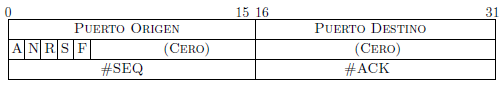
\includegraphics[width=\textwidth,keepaspectratio]{formatosegmento.png}
\end{center}
\caption{Formato del encabezado de PTC} \label{figura1}
\end{figure}

Los campos A, N, R, S y F, todos de 1 bit, representan los flags:

\begin{itemize}
	\item A es el flag de ACK; prendido s'olo en los mensajes del servidor para reconocer la correcta recepci'on de un paquete.
	\item S es el flag de SYN; es enviado s'olo por el cliente al requerir establecer una nueva conexi'on.
	\item F es el flag de FIN; es enviado 'unicamente por el cliente cuando desea finalizar una conexi'on existente.
	\item Los flags N y R actualmente no tienen uso.
\end{itemize}	

Inmediatamente despu'es de este encabezado siguen los datos, de longitud arbitraria aunque entre 1 y 1000 bytes. El n'umero de secuencia no trabaja a nivel de byte como ocurre en TCP sino que identifica a toda la porci'on de los datos contenida en el paquete. As'i como un segmento TCP se encapsula dentro de un datagrama IP, los paquetes de PTC tambi'en viajar'an dentro de IP. Para que los hosts puedan reconocer este hecho, el campo proto del header IP debe definirise
con valor 202, tradicionalmente sin uso (el protocolo TCP se identifica con el valor 6). 

\subsection {Establecimiento y liberaci'on de conexi'on}

Antes de poder enviar sus datos, el cliente debe establecer activamente una conexi'on con el servidor deseado. Para ello, debe enviar un segmento con el flag SYN prendido y con un valor arbitrario en el campo \#SEQ que indique el n'umero de secuencia inicial que utilizar'a el cliente para identificar sus paquetes. El resto de los campos pueden tener un valor arbitrario; no ser'an tenidos en cuenta por el servidor. Por su parte, el servidor responder'a con un segmento con el flag ACK prendido y el campo \#ACK reconociendo el valor de \#SEQ previamente recibido. Una vez hecho esto, el servidor considerar'a que la conexi'on está establecida. Lo mismo har'a el cliente al recibir este reconocimiento. En caso de no llegar, el cliente eventualmente retransmitir'a el paquete inicial. Se observa que no se requiere un SYN por parte del sevidor: al no enviar datos, no es necesario que 'este sincronice su n'umero de secuencia con el cliente. Para cerrar la conexi'on, la secuencia a seguir es similar, aunque cambiando el flag de SYN por el flag de FIN. El segmento FIN enviado por el cliente tambi'en debe ir secuenciado como cualquier otro segmento de datos previamente enviado. En caso de no recibir el ACK respectivo, el cliente tambi'en retransmitir'a el FIN.

\subsection{Ventana deslizante y retransmisiones}

Para garantizar la confiabilidad, PTC implementa ventana deslizante, particularmente GoBackN[1]. De esta manera, el servidor tiene una ventana de recepci'on de tamaño 1, mientras que el cliente tiene una ventana de emisi'on de tamaño que por simplicidad se fija en un valor constante arbitrario (potencialmente mayor que
1). Llamaremos \texttt{SEND\_WINDOW} a este valor. El cliente, entonces, podr'a enviar hasta \texttt{SEND\_WINDOW} paquetes en simult'aneo antes de bloquearse esperando por los sucesivos reconocimientos. Cada ACK recibido permitir'a desplazar la ventana y as'i hacer lugar para el env'io de nuevos segmentos. Adem'as, los ACKs del servidor pueden ser acumulativos (i.e., un paquete ACK puede reconocer m'as de un paquete con n'umeros de secuencia contiguos enviados por el cliente).

Al enviar un segmento con datos, el cliente tambi'en encolar'a este segmento en la cola de retransmisi'on. 'Este permanecer'a all'i hasta ser eventualmente reconocido. Por otro lado, el cliente tambi'en define un tiempo m'aximo de espera \texttt{RETRANSMISSION\_TIMEOUT} para esperar por estos reconocimientos. De superarse este tiempo, se asumir'a que el paquete se extravi'o en los rincones de la red y por ende ser'a retransmitido junto con todo segmento posterior aguardando en la cola de retransmisi'on.

Se define tambi'en un n'umero m'aximo admisible de retranmisiones, \texttt{MAX\_RETRANSMISSION\_ATTEMPTS}. Si alg'un segmento del cliente debiera ser retransmitido m'as veces que esta cantidad, se debe asumir que la conexi'on se perdi'o, y se pasar'a a cerrarla sin enviar FIN. 

\subsection{Estados}

En lo que sigue veremos los posibles estados que pueden atrevesar tanto el cliente como el servidor:

Estados del cliente:

\begin{itemize}
	\item CLOSED: Representa la ausencia de conexi'on (Estado anterior: FIN\_SENT o ninguno)
	\item SYN\_SENT: El cliente desea iniciar una conexi'on y ha enviado un SYN (Estado anterior: CLOSED)
	\item ESTABLISHED: El cliente recibi'o el ACK del SYN y ya puede enviar datos. (Estado anterior: SYN\_SENT)
	\item FIN\_SENT: El cliente desea terminar la conexi'on y ha enviado un FIN al servidor (Estado anterior: ESTABLISHED)
\end{itemize}

Estados del servidor: 

\begin{itemize}
	\item CLOSED: Representa la ausencia de conexi'on (Estado anterior: FIN\_RECEIVED o ninguno)
	\item SYN\_RECEIVED: El servidor recibi'o un SYN y debe enviar el ACK respectivo (Estado anterior: CLOSED)
	\item ESTABLISHED: El servidor ha enviado el ACK y est'a a la espera de recibir datos (Estado anterior: SYN\_RECEIVED)
	\item FIN\_RECEIVED: El servidor recibi'o un FIN y debe enviar el ACK respectivo (Estado anterior: ESTABLISHED)
\end{itemize}